%======================================%
% Subfile                              %
%======================================%

% Template

\section{Übersicht}

Fallschirm für Drohnen. Bei Ausfall des Flugsystems wird die Drohnen sicher mittels Fallschirmes gelandet. Die Drohnen transportiert fragile Ware und darf deshalb zu keinem Zeitpunkt einfach abstürzen.

\section{Implementation}

\subsection{Hardware}

\begin{itemize}
	\item Beschleunigungssensoren (xyz), mehrere Redundant, ungerade Anzahl z.B. 3x
	\item Mikrokontroller (3 verschiedene (z.B. 1xRisc-V, 1xCortex-M4, FPGA) )
	\item Energieversorgung, doppelt ausgeführt.
\end{itemize}

\subsection{Software}
\begin{itemize}
	\item FPGA implementiert mit VHDL
	\item 1× MCU programmiert in C, kompiliert mit GCC
	\item 1× MCU programmiert in C++, kompiliert mit TI-CX2000
	\item Mehrheitsentscheid über Sensorwerte: Wenn 2 von 3 freien Fall melden, wird der Fallschirm ausgelöst
	\item Prozessoren laufen jeweils um einen Taktzyklus versetzt
	\item Wenn ein Fallschirm ausgelöst wurde und keine Bremsbeschleunigung detektiert wird: Zündung eines zweiten Fallschirms
\end{itemize}

\subsection{Aktor}
\begin{itemize}
	\item Sprengkapsel, die den Fallschirm enthält und auslöst (2 Stück)
	\item \url{https://shop.thebioniceye.co.uk/products/gbs50}
	\item Galaxy Sky Ballistic Parachutes
	\item Bedingung: Bekannter Lieferant mit viel Erfahrung in diesem Gebiet (geringes Risiko, dass unerfahrener Hersteller \textit{Anfängerfehler} macht.)
\end{itemize}



\begin{figure}[H]
	\begin{center}
		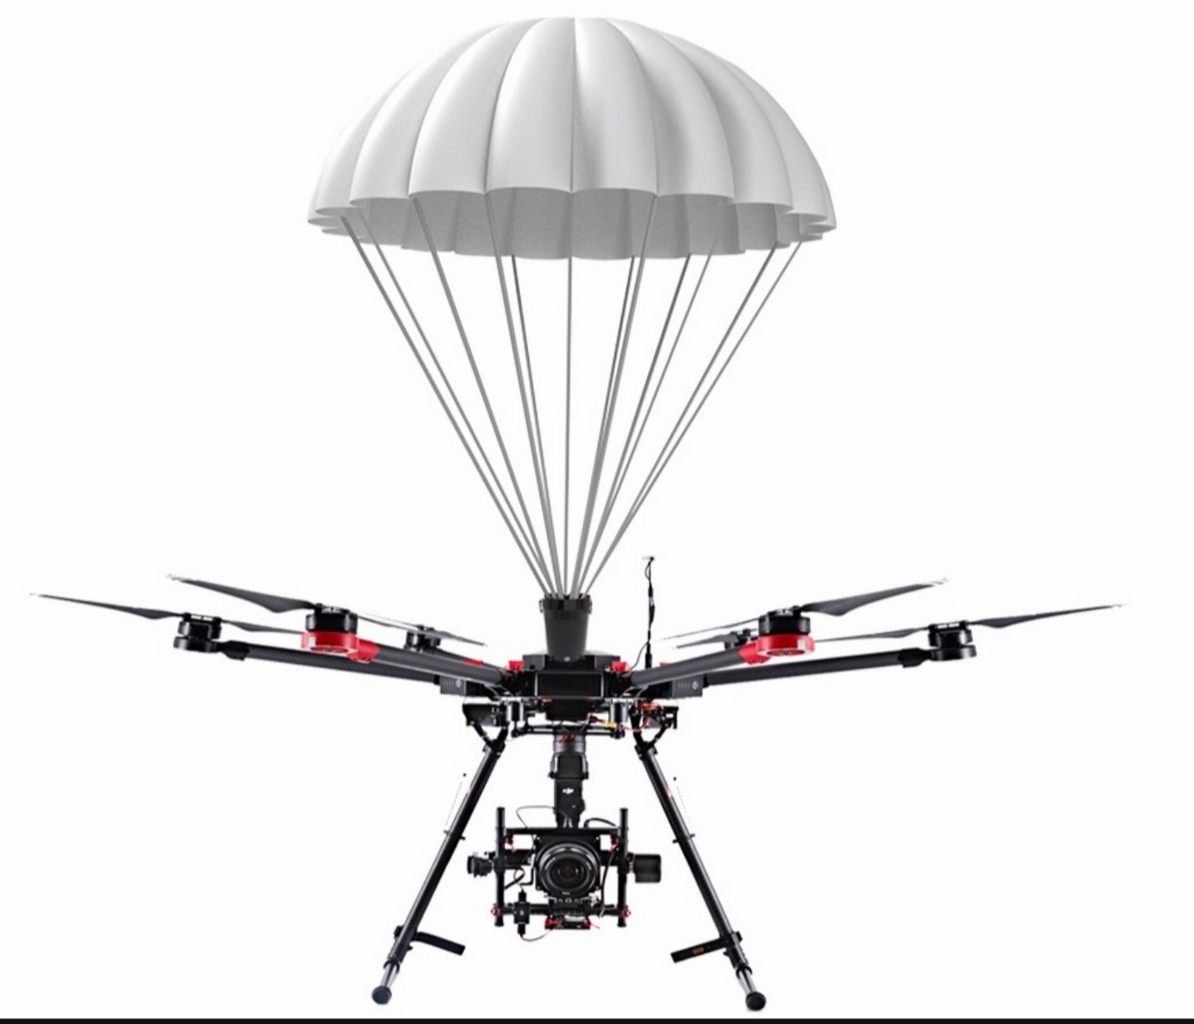
\includegraphics[width=0.3\textwidth]{mainmatter/figures/bild_fallschirm.png}
	\end{center}
	\caption{Quelle: {\tiny \url{https://www.uavgl.com/quality-12710049-smart-drone-parachute-system-for-commercial-drone-safety-10-100kg-load-capacity}}}
\end{figure}

\subsection{Fehlerquellen}
\begin{itemize}
	\item Starke EMI könnte zu messfehlern mehrerer accelerometer führen
	\item Überhitzung der Aktoren führt zu ungewollter Auslösung der Fallschirme
	\item Distanz zum Boden ist bei Auslösung kleiner als 5m (vorgabe des Fallschirmes)
	\item Fehlfunktion der Drohne fürt zu Position, in welcher der Fallschirm nicht ausgelöst werden kann (Drohne Verliert Propeller und Dreht sich um 180° in X oder Y Achse)
    \item Rotoren Drehen sich nach dem Abschalten noch schnell genug, um den Ersten Fallschirm zu beschädigen, oder zu zerstören.
    \item unzureichende Redundanz, es fallen mehr Teile (Sensoren, Prozessoren, etc) aus, als eingeplant wurden.
    \Item Accelerometer werden duch zu Starke beschleunigungen beschädigt (unwahrscheinlich oft für mehrere tausend G ausgelegt)
\end{itemize}

\subsection{Schema}
\begin{figure}[H]
	\begin{center}
		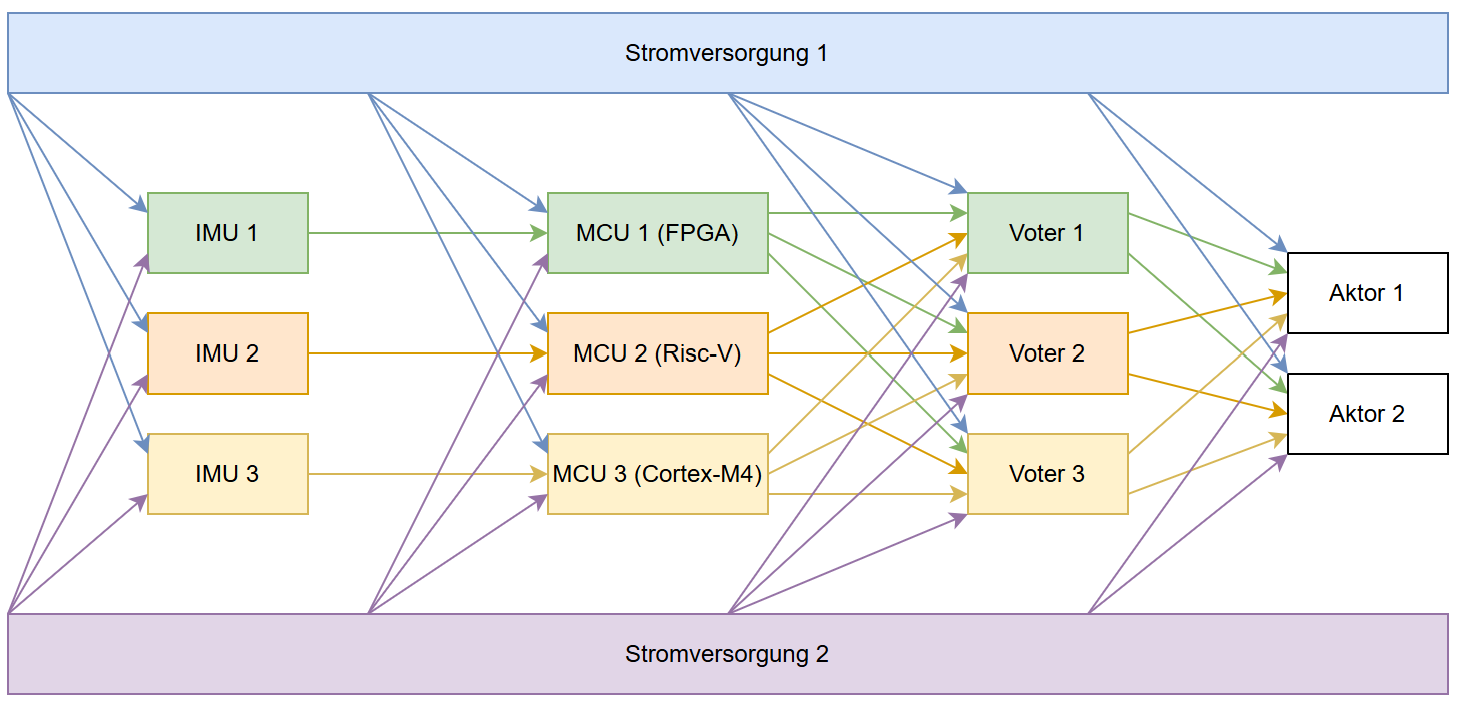
\includegraphics[width=\textwidth]{mainmatter/figures/schema.png}
	\end{center}
	\caption{ Schematische Darstellung des Fallschirm-Systems}
\end{figure}